\section{Transfer}
\label{sec:transfer}
Una volta ottenuto l'albero di parsing per la frase nella lingua sorgente,
dobbiamo disporre di opportune regole/fonti di conoscenza che ci consentano di attuare 
il Transfer lessicale e sintattico.
\subsection{Transfer lessicale}
Denotiamo con $I$ il lessico \ref{lexicon} dichiarato nella Sottosezione \ref{sec:requisiti}.Possiamo notare come non tutti i lemmi siano monosemici. Il caso più evidente è dato dal verbo polisemico "fare", il quale in relazione al contesto può assumere un significato (\textit{senso}) differente. In Figura vengono riportate due possibili accezioni ottenute consultando la risorsa Babelnet, che evidenziano come la traduzione debba avvenire sulla base del particolare senso del lemma. 
	\begin{figure}[ht]
		\centering
		\begin{subfigure}{.5\textwidth}
			\centering
			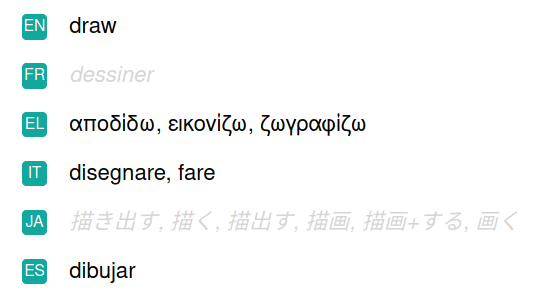
\includegraphics[width=1\linewidth]{./img/fare_synset1.png}
			\caption{Gloss: Drawing an artifact}
			\label{fig:sub1}
		\end{subfigure}%
		\begin{subfigure}{.5\textwidth}
			\centering
			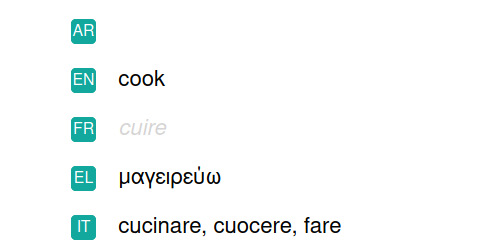
\includegraphics[width=1\linewidth]{./img/fare_synset2.png}
			\caption{Gloss: Transform and make suitable for consumption by heating}
			\label{fig:sub2}
		\end{subfigure}
		\caption{Due Babel-synset in cui compare il lemma "fare". In ogni synset, BabelNet fornisce l'elenco di sinonimi nelle varie lingue ed una definizione (Gloss) del significato sotteso}
		\label{fig:test}
	\end{figure}

Per evitare di dover svolgere Word Sense Disambiguation e quindi di dover analizzare il contesto in cui la parola occorre, sono state fatte le seguenti ipotesi semplificative:
\begin{itemize}
	\item I termini polisemici i cui lemmi appartengono ad $I$ assumono un significato definito a priori e non dipendente dal contesto 
	\item La \textbf{traduzione} dei lemmi è una relazione funzionale ed ovunque definita $R$  tra gli elementi di $I$ ed i lemmi della lingua inglese appartenenti all'insieme denotato con $E$. Ovvero vale la seguente condizione:
	\begin{align*}
		\forall x \in I \quad  \exists! y \in E \quad t.c. \; (x,y) \in R 
	\end{align*}
\end{itemize}
In questo modo per la traduzione possiamo ricorrere ad un dizionario isomorfo italiano-inglese, implementabile in Java con un HashMap.
	\lstinputlisting[label={dizionario},style = javacode, caption ={Dizionario isomorfo IT->EN}]{java/Dizionario}  
Nel Transfer lessicale, visitiamo ciascun nodo dell'albero tramite ricerca in ampiezza, ed estraiamo il lemma della parola associata al nodo. \\
In generale, viene tradotto direttamente l'intero lemma utilizzando il dizionario sopra definito.
Tuttavia, nel caso in cui la parola fosse una preposizione, anziché tradurre direttamente l'intero lemma, traduciamo i morfemi con l'uso del suddetto dizionario e poniamo uno spazio tra i morfemi tradotti per generare il risultato.
Ad esempio, data la preposizione "della", individuiamo i morfemi "del-la" derivanti dall'analisi morfologica. Traduciamo quindi i singoli morfermi (del->of, la->the) in modo da ottenere la traduzione "of the". \\
Il risultato della traduzione viene salvato in un attributo del nodo corrente visitato.
\subsection{Transfer sintattico}
\label{sec:transfer_sintattico}
Il processo di generazione, che rappresenta la fase finale della nostra pipeline di elaborazione (Fig. \ref{Vauquois_triangle}), è affidato alla libreria Java SimpleNLG \cite{simpleNLG}, un \textbf{realizzatore linguistico} che utilizzando regole grammaticali dell'inglese (morfologiche e sintattiche) converte la rappresentazione astratta della frase (\textbf{sentence plan ibrido}) data in input in testo effettivo. \\

Pertanto, nel nostro caso il ruolo del Transfer Sintattico è quello di fungere da ponte tra l'albero a dipendenze finora discusso ed il sentence plan ibrido richiesto in input da SimpleNLG.
\begin{figure}[ht]
	\centering 
	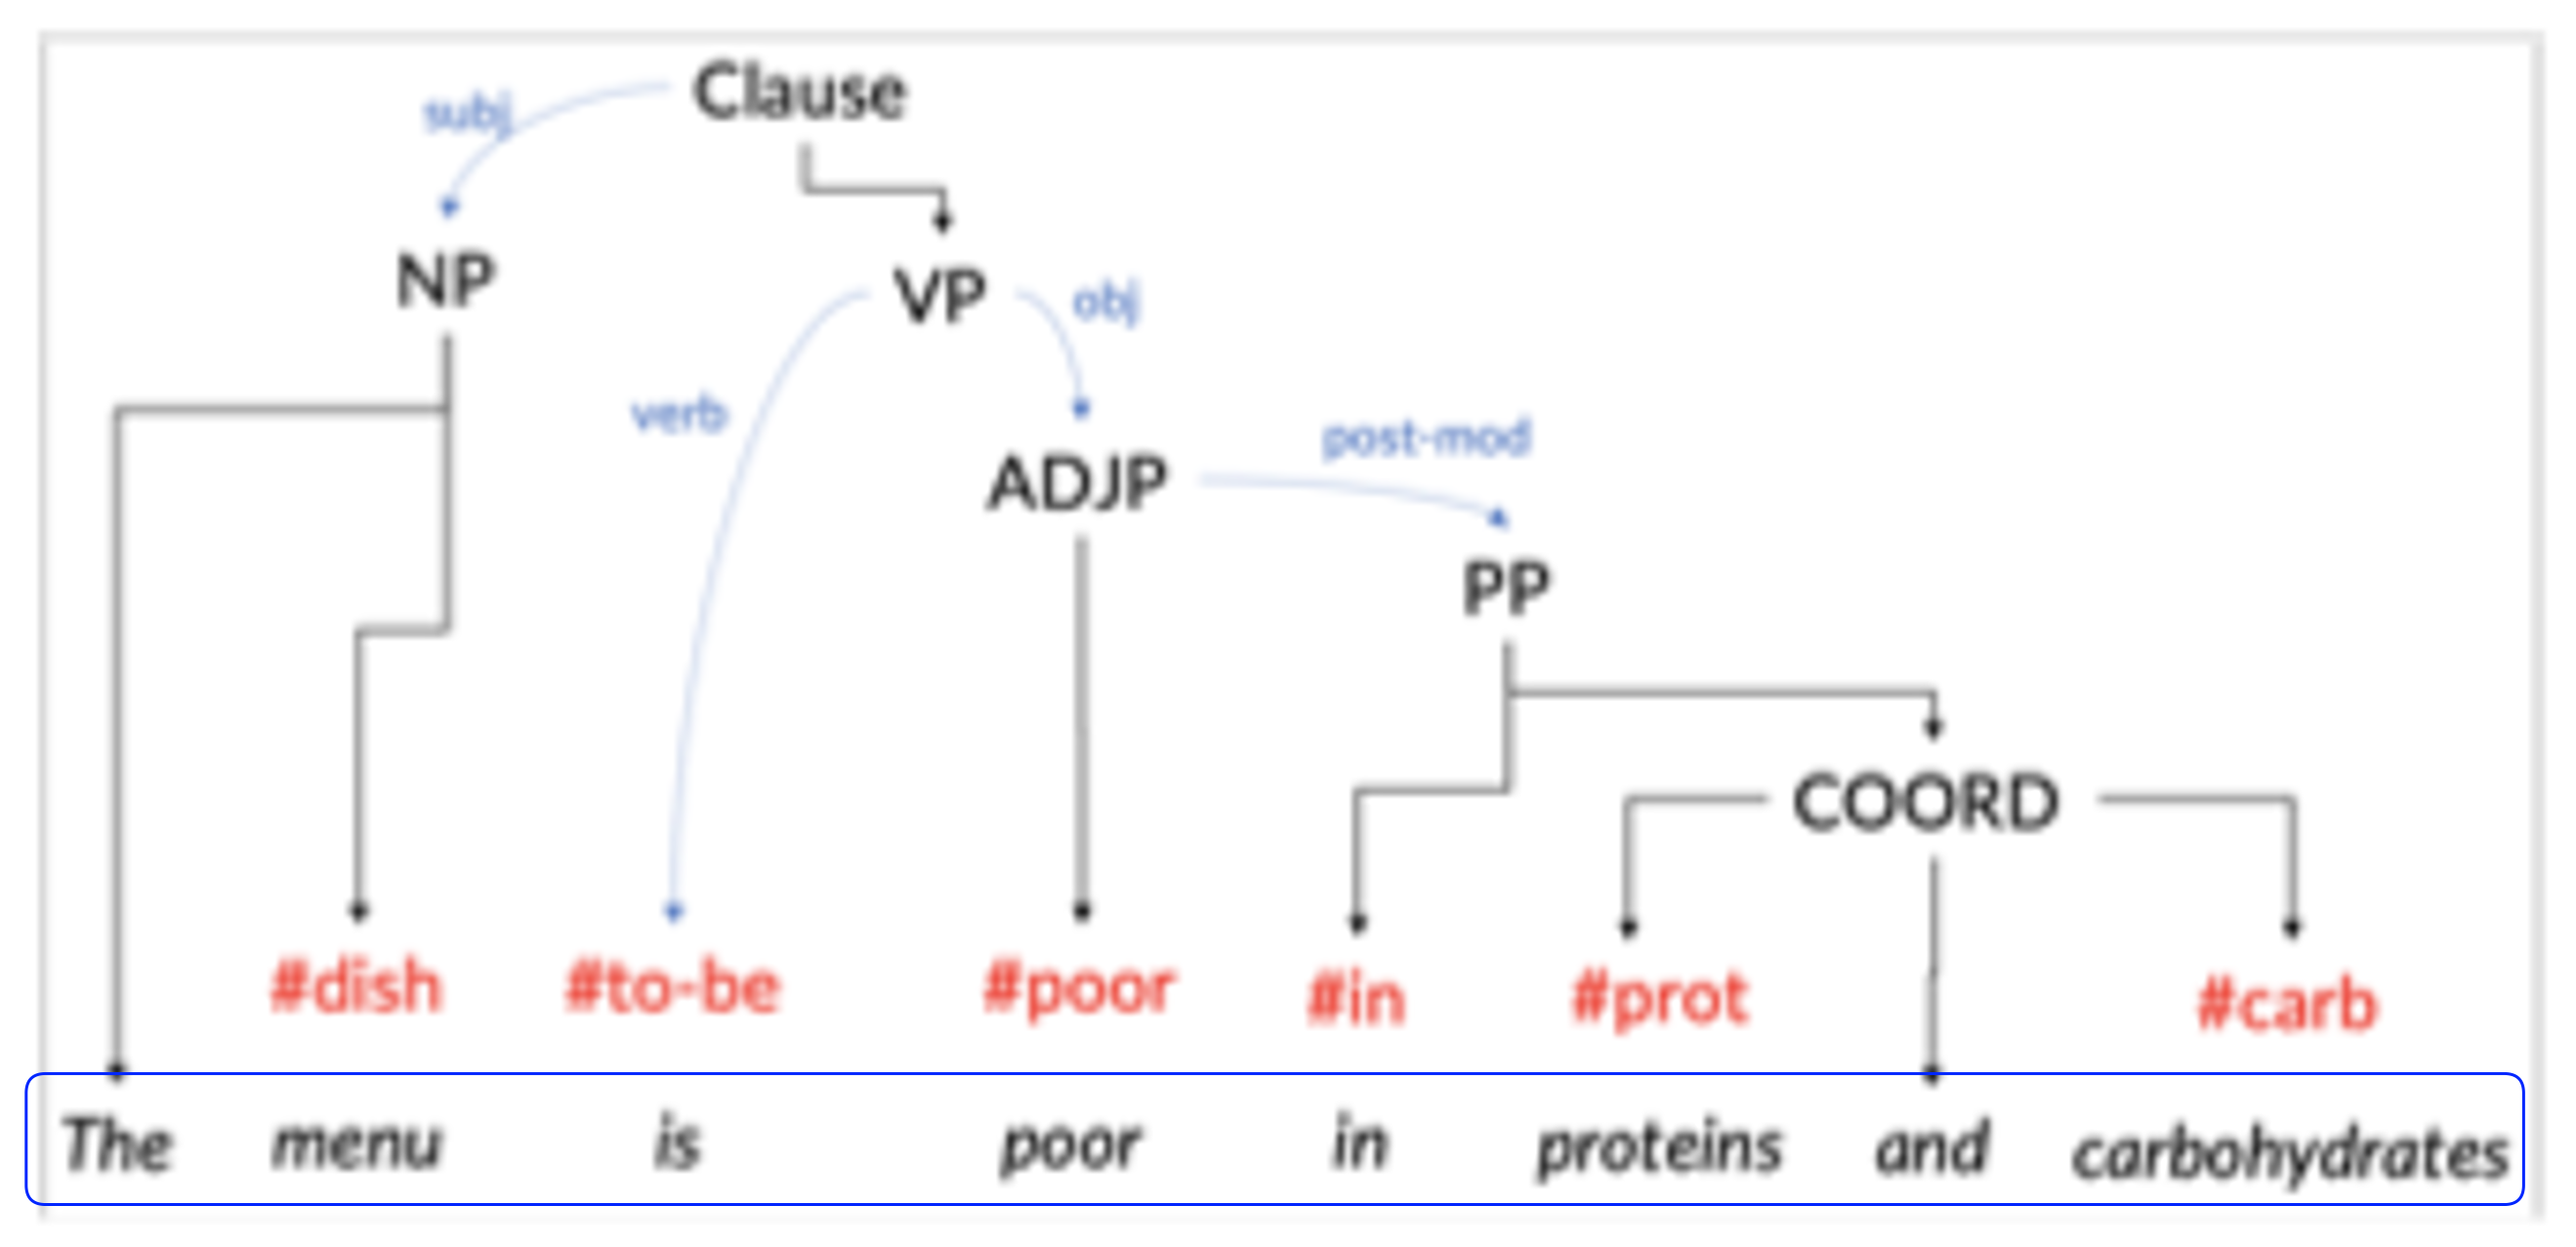
\includegraphics[width=1\linewidth]{./img/sentence_plan}
	\caption{Nella parte alta viene raffigurato un sentence plan ibrido, nell'ultimo livello viene presentato il risultato della realizzazione linguistica (testo)}
	\label{sentence_plan}
\end{figure} \\
Ci limitiamo a fare alcune considerazioni sulle peculiarità di quest'ultima struttura dati citata, considerando l'esempio in Figura 5:
\begin{itemize}
	\item Vi sono relazioni binarie asimmetriche grammaticali tra la frase ed i costituenti. \\Nell'esempio la relazione \textit{subj} lega la frase ad un NP (sintagma nominale)
	\item Si può specificare relazioni binarie asimmetriche grammaticali anche tra i costituenti. \\Nell'esempio la relazione \textit{post-mod} lega il sintagma aggettivale (dominante) ad un PP (modificatore ).	
	\item Le foglie dell'albero ospitano i lemmi in lingua inglese. Sarà compito di SimpleNLG effettuare la generazione morfologica sulla base delle informazioni linguistiche fornite (ad esempio, se il soggetto è in terza persona singolare ed il tempo verbale è al presente, verrà aggiunto il suffisso "-s" al verbo)
	\item In questa rappresentazione astratta della frase, l'ordine delle parole non c'è in quanto sarà stabilito da SimpleNLG al momento della generazione, in maniera conforme alle regole morfo-sintattiche dell'inglese
\end{itemize}
		\begin{figure}[ht]
		\centering
		\begin{subfigure}{.4\textwidth}
			\centering
			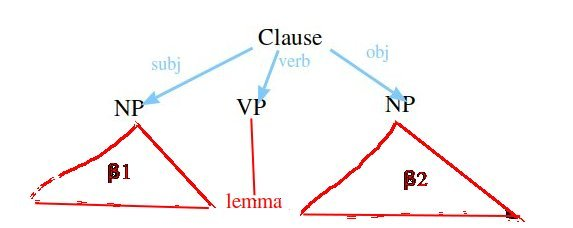
\includegraphics[width=1\linewidth]{./img/fase2_transfer}
			\caption{Sentence plan ibrido}
			\label{fig:tree_transfer}
		\end{subfigure}%
		\begin{subfigure}{.6\textwidth}
			\centering
			\lstinputlisting[label={transfer},style = javacode, caption ={}]{java/Fase2Transfer.java}  
			\caption{Snippet di codice costruzione sentence-plan ibrido a partire dall'albero a dipendenze}
			\label{fig:code_transfer}
		\end{subfigure}
		\caption{Da una parte porzione del codice utilizzato per trasformare l'albero a dipendenze in un sentence plan. Dall'altra rappresentazione grafica della struttura dati generata. }
		\label{fig:transfer}
	\end{figure}
Descriviamo ora il processo di trasformazione dell'albero a dipendenze in sentence plan ibrido,
supponendo che la frase in ingresso sia in forma attiva e che il verbo sia transitivo\footnote{NOTA BENE: per rendere l'esposizione più chiara, la descrizione si è focalizzata al caso in cui la frase fosse attiva ed il verbo transitivo. Tuttavia, il programma dispone di opportune regole per gestire casi relativi a frasi in forma passiva, predicati nominali, ... etc.}.. \\

In primo luogo, si esaminano i nodi dell'albero a dipendenze posti ad una profondità massima di 1 per determinare le relazioni grammaticali della frase (\textit{subj}, \textit{verb}, \textit{obj}) che sono di interesse per il sentence plan ibrido (Figura \ref{fig:transfer} (a)).
Ognuna di queste relazioni coinvolge un opportuno costituente: si costruisce il sotto-albero sotteso (nell'esempio $\beta_1$ per il soggetto, $\beta_2$ per il complemento oggetto) richiamando la funzione  \textit{generatePhrase} (Listing \ref{fig:transfer} (b)) passandogli il nodo dell'albero a dipendenze appena visitato. La funzione tratta tale nodo come una radice di un sotto-albero, che verrà visitato nell'ottica di ottenere le informazioni utili per generare il sotto-albero del sentence plan ibrido.
\\Inoltra, una peculiarità della funzione \textit{generatePhrase} è quella di riuscire a gestire la seguente ricorsione:
			\[ NP \longrightarrow Det \; Noun \;PP \; | \; Det \; Noun \]
			\[ PP \longrightarrow Prep \; NP  \]	
\begin{figure}[ht]
	\centering 
	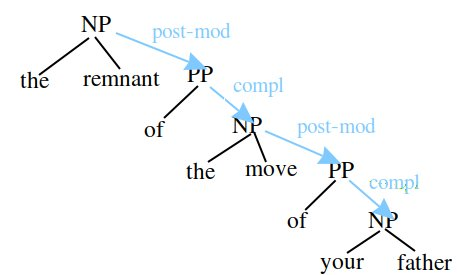
\includegraphics[scale=0.5]{./img/ricorsione}
	\caption{Struttura ricorsiva nel sentence plan ibrido}
	\label{sentence_plan}
\end{figure}
Una volta costruito il sentence plan, SimpleNLG si occuperà di generare la frase per l'inglese, come già discusso all'inizio di questa sezione.

		
							






